\section{AutoLibra as a ladder \protect\includegraphics[height=1em]{figs/ladder.png}: Agent improvement with AutoLibra}
\label{sec:ladder}

As AutoLibra can automatically induce metrics from human feedback, a natural question to ask is whether it can enable self-regulated improvement in agents through iterative feedback. 
In this section, we will study can AutoLibra be used a `ladder', inducing metrics as new optimization targets in each iteration to improve agent performance. We investigate two methods for optimizing agents:
prompt engineering and fine-tuning, across two domains: text game and web browsing. Across all tested methods and domains, AutoLibra induces new metrics in each iteration to cover emergent agent behaviors, and enables continuous improvements on both induced metrics and task success.
Fig. \ref{fig:autolibra-training} illustrates the results. 

\begin{figure}[!t]
    \centering
    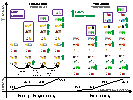
\includegraphics[width=0.8\textwidth]{figs/autolibra-teaser.pdf}
    \caption{AutoLibra iteratively discovers new optimization targets throughout the agent optimization process. Each emoji pair represents a metric; the text between iterations in prompt engineer experiment represents the improvement in the prompts. Purple boxes indicate the new emerging metrics, and green arrows indicate significant improvements over the previous iteration. The metric names can be found in Tab. \ref{tab:baba_is_ai_metrics} and App. Tab. \ref{tab:app_nnetnav_metrics}.
    }
    \label{fig:autolibra-training}
\end{figure}

\subsection{Can AutoLibra induce good optimization targets for prompt engineering?}
\label{sec:Baba-Is-AI}

To answer this question, we use Baba-Is-AI \citep{cloos2024babaaibreakrules, paglieri2024balrog} as a case study, since it is a challenging environment not yet saturated by state-of-the-art LLM agents. This game requires metacognitive skills, such as breaking and building new rules, planning ordered subtasks, and advanced navigation. A full list of game rules is listed in App. \ref{appendix:baba_is_ai_rules}.
We use the top model on the leaderboard\footnote{\url{https://balrogai.com}} (which when we started the experiments, was GPT-4o) \citep{openai2024gpt4ocard} for the agent policy, while we find similar improvements in Claude-3.5-Sonnet\footnote{\url{https://www.anthropic.com/news/claude-3-5-sonnet}} as well.

% \begin{figure}[ht]
%     \centering
%     \includegraphics[scale=0.5]{figs/babaisai_env.png}
%     \caption{Example of the Baba-Is-AI environment. In this task (two\_room-break\_stop-make\_win-distr\_obj-irrelevant\_rule), the agent has to break the "wall is stop" rule and push the "key" rule block next to "is win" to assemble the win rule, then touch the key to win. Pushing the "door" rule block would be a mistake, as no door object is present.}
%     \label{fig:babaisai_env}
% \end{figure}

% \subsection{AutoLibra for Baba-Is-AI improvement}

To avoid overfitting to the tasks used in optimization, we use 6 of 40 tasks in Baba-Is-AI \citep{paglieri2024balrog} to induce metrics and optimize prompts and report performance on all 40 tasks. 
In one \textit{Iteration}, the human prompt engineers (two of the authors) generate 18 agent trajectories (3 trajectories / task), use AutoLibra to induce metrics, then optimize the prompt to achieve higher performance on the induced metrics without considering the task success rate, and start a new iteration when one or more metrics improved significantly (over 30\%). The procedure and experiment setup are detailed in App. Alg. \ref{appendix:algo1} and App. \ref{appendix:autolibra_setup}.

\paragraph{Results}
Illustrated in Fig. \ref{fig:autolibra-training}, the performance on Babaisai task increased from 25\% to 55\% between \textit{Iteration 0} and \textit{Iteration 3}, with each iteration resulting in greater performance than the previous; this is replicated across the held-out tasks alone, (complete task results tabulated in App. \ref{appendix:heldout}). This represents a substantial increase compared to the highest base model performance of 33\% on Baba-Is-AI \citep{paglieri2024balrog}. With only 6 tasks used in inducing the metrics, the improvement on all 40 tasks showing the metrics induced by AutoLibra are generalizable to unseen tasks. Among induced metrics (App. Tab. \ref{tab:baba_is_ai_metrics}), agent performance increases correspondingly to prompt changes targeting those metrics, an example being \texttt{Win Condition Recognition} \includegraphics[height=1em]{figs/emojis/emoji_1.png}, which increases from 28\% to 50\% from \textit{Iterations 0-1} after few-shot prompting (prompt in App. \ref{box:baba_is_you_iter_1}) is introduced to teach the identification of a win condition rule. The complete list of observations and reasoning for prompt engineering is in the App. \ref{appendix:baba_is_ai_obs}. With AutoLibra, prompt engineers could receive feedback on whether their prompt changes lead to desired behavior changes in agents. 

\begin{wraptable}[20]{r}{0.60\textwidth} % 'r' for right, adjust the width as needed
\centering
\small
\vspace{-10pt}
\begin{tabular}{ccl}
\toprule
\multicolumn{1}{c}{Emoji}& 
\multicolumn{1}{c}{It.} & 
\multicolumn{1}{l}{Metric} \\
\midrule
\rowcolor{gray!10} \includegraphics[scale=0.07]{figs/emojis/emoji_1.png} & 0 & Win Condition Recognition \\
\midrule
\rowcolor{gray!10} \includegraphics[scale=0.07]{figs/emojis/emoji_2.png} & 0 & Rule Modification \\
\midrule
\rowcolor{gray!10} \includegraphics[scale=0.07]{figs/emojis/emoji_3.png} & 0 & Direct Navigation Efficiency \\
\midrule
\rowcolor{gray!10} \includegraphics[scale=0.07]{figs/emojis/emoji_4.png} & 0 & Context-Sensitive Decision Making \\
\midrule
\rowcolor{gray!30} \includegraphics[scale=0.07]{figs/emojis/emoji_5.png} & 1 & Win Rule Construction \\
\midrule
\rowcolor{gray!30} \includegraphics[scale=0.07]{figs/emojis/emoji_6.png} & 1 & Selective Interaction With Relevant Objects  \\
\midrule
\rowcolor{gray!30} \includegraphics[scale=0.07]{figs/emojis/emoji_7.png} & 1 & Rule Manipulation and Execution  \\
\midrule
\rowcolor{gray!60} \includegraphics[scale=0.07]{figs/emojis/emoji_8.png} & 2 & Subtask Coordination \\
\midrule
\rowcolor{gray!90} \includegraphics[scale=0.07]{figs/emojis/emoji_9.png} & 3 & Immovable Interaction \\
\bottomrule
\end{tabular}
\caption{Metrics and Turn of Induction \newline for Baba-Is-AI}
\label{tab:baba_is_ai_metrics}
\end{wraptable}

% Similarly to results observed in Section 3, induced metrics are observed to capture the behavior of the agent increasingly well with additional iterations, with coverage increasing from 65\% at \textit{Iteration 0} to 92\% at \textit{Iteration}, while mean redundancy remains 56\% across all iterations. The trajectory performance also improved significantly, with the average number of steps per task (capped at 100) decreasing from 79 to 51, indicating that the agent's reasoning performance and efficiency improved as a result of the code changes made in each iteration.

Qualitative observation of agent trajectories reveals behaviors commensurate with induced metric scores; the agent random-walks in \textit{Iteration 0}, navigates towards specific objectives but gets stuck or trapped in a loop on long-horizon tasks in \textit{Iteration 1} and \textit{Iteration 2}, and fully understands basic subtasks (atomic goals on the critical path to environment completion) and the correct order of subtasks to successfully complete an environment in \textit{Iteration 3}. A per-metric score breakdown is listed in Appendix \ref{appendix:babaisai}, and a full per-iteration documentation of code changes and results is presented in Appendix \ref{appendix:baba_is_ai_obs}.

% \subsubsection{Held-Out Task Performance}

% \paragraph{Ablation Study}

% To evaluate the generalization of the improvements realized by AutoLibra, we conducted an ablation study where the performance of the agent improved by AutoLibra was evaluated on unseen Baba Is You levels, arbitrary LLMs, and entirely new environments.

\textbf{Generalization to other models} When replacing GPT-4o with Claude-3.5 as the LLM used in the agent (Appendix \ref{appendix:heldout}), performance was found to be similar across all iterations, with held-out task performance increasing by 20\% to 55\% between \textit{Iteration 0} and \textit{Iteration 3} and qualitatively similar trajectory performance and agent behaviors observed between the two LLMs. This demonstrates that the improvements realized by AutoLibra are generalizable to other LLMs, and that the induced metrics are robust to changes in the underlying LLM.

\textbf{Generalization to other tasks} To evaluate whether this pipeline can be generalized to other domains, we conduct the same pipeline to MiniHack \citep{samvelyan2021minihackplanetsandboxopenended}, an environment whose tasks and action space are more complex than Baba-Is-AI. Similarly to Baba-Is-AI, in three iterations, the task completion rate was observed to increase to 25\%, an improvement of 15\% versus the baseline of 10\%, validating AutoLibra's general utility in improving agent performance; full results are available in the Appendices \ref{appendix:minihack_rules}-\ref{appendix:minihack_obs}.
%\diyi{use a paragraph title to illustrate that this is about generalization? i also didn't quite follow why minihack is only summarized using these two sentences. if you want to emphasize it, explain it clearly; otherwise, no need to mention it? } 


\subsection{Can AutoLibra induce good optimization targets for agent fine-tuning?}
\label{sec:webvoyager}
To answer this question, we use web browsing as the case study domain, as we can compare the effectiveness of AutoLibra with the existing goal-oriented LLM-as-a-Judge method in rejection behavior cloning methods for agent fine-tuning.
Previously, we collected a diverse dataset (NNetNav-live) of agent trajectories through open-end exploration on 20 live websites, which were labeled with tasks in the hindsight \citep{Murty2025NNetNav}. 
Through this process, the tasks in NNetNav-live have no overlap and are more complex than the evaluation datasets that we use in this subsection, WebVoyager \citep{he2024webvoyager}.
We start from the state-of-the-art agent Llama-8b-nnetnav-live, which was finetuned with trajectories selected with LLM-as-a-Judge instructed to evaluate trajectories based on goal completion. Following a similar pipeline in \S\ref{sec:Baba-Is-AI}, we improve the agents for 3 iterations, and get feedback on 18 trajectories in each iteration. The difference is that instead of prompt engineering, we use the induced metrics to choose the sampled trajectories with top 10\% sum scores of all metrics for fine-tuning the agent policy. Throughout the training procedure, we use the tasks in NNetNav-live \citep{Murty2025NNetNav} for metric induction and agent finetuning. This process yields the continuous improvement on WebVoyager \citep{he2024webvoyager}, shown in Fig. \ref{fig:autolibra-training}. In contrast, using LLM-as-a-Judge instructed to evaluate goal completion does not yield significant improvement even for one iteration. This shows that the metrics iteratively induced by AutoLibra also serve as better optimization target than the goal-oriented evaluation metric alone. Metrics induced in each iteration are in App. Tab. \ref{tab:app_nnetnav_metrics}.